\section{De klasse Tijdsduur.}

We willen een ADT (Abstract Data Type), oftewel een 'zelfgedefinieerd datatype' maken waarin een tijdsduur in minuten en seconden kan worden opgeslagen. De totale tijd in seconden kan ook worden opgevraagd. 
\begin{figure}[h!]
	\captionsetup{justification=centering}
	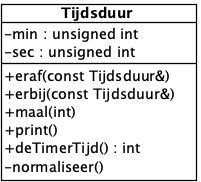
\includegraphics[width=0.28 \linewidth]{figuren/tijdsduur}
	\centering
	\caption{weergave van de klasse Tijdsduur. }
	\label{fig:tijdsduurKlas}
\end{figure}
We noemen dit zelf gedefinieerde datatype \texttt{Tijdsduur}. Figuur \ref{fig:tijdsduurKlas} geeft de klasse weer van Tijdsduur.
Het ADT \texttt{Tijdsduur} kan in C++ als volgt gedeclareerd worden in de header file (tijdsduur.h):

\begin{lstlisting}[caption= de headerfile van de klasse \texttt{Tijdsduur},label={lst:tijdsdHeader},numbers=none]		
	#ifndef TIJDSDUUR_H
	#define TIJDSDUUR_H
	
	// De declaratie van de ADT Tijdsduur:
	class Tijdsduur {
		public:
		//...
		void eraf(Tijdsduur t);
		//...
		
		private:
		int sec;
		//...
	};
	#endif // TIJDSDUUR_H
\end{lstlisting}
\newpage
De implementatie (\texttt{tijdsduur.cpp}) ziet er tot nu toe als volgt uit:
\begin{lstlisting}[caption= de implementatiefile van de klasse \texttt{Tijdsduur},label={lst:tijdsdImpl},numbers=none]
	#include <iostream>
	#include "tijdsduur.h"
	#include <iomanip>
	using namespace std;
	
	// De definities van de memberfunctie van de ADT Tijdsduur, oftewel: de implementatie van de ADT Tijdsduur:
	void Tijdsduur::eraf(Tijdsduur t) {
		sec-=t.sec;
		//...
	}
\end{lstlisting}

Het hoofdprogramma (\texttt{testTijdsduur.cpp}) ziet er als volgt uit:

\begin{lstlisting}[caption= de implementatiefile van het hoofdprogramma ,label={lst:tijdsdMainprog},numbers=none]
	#include <iostream> // nodig voor cout (schrijven naar scherm)
	#include <iomanip> // nodig voor setw (veldbreedte definieren )
	#include "tijdsduur.h"
	using namespace std;
	
	int main() {
		Tijdsduur t1(3,50); // t1 is 3 minuten en 50 seconden
		cout<<"t1 = "; t1.print(); cout<<endl;
		const Tijdsduur kw(15); // kw is 15 seconden
		cout<<"kw = "; kw.print(); cout<<endl;
		t1.erbij(kw); // Tel kw bij t1 op
		cout<<"t1 = "; t1.print(); cout<<endl;
		Tijdsduur t2(t1); // t2 is een kopie van t1
		t2.eraf(kw); // Trek kw van t2 af
		cout<<"t2 = "; t2.print(); cout<<endl;
		t2.maal(7); // Vermenigvuldig t2 met 7
		cout<<"t2 = "; t2.print(); cout<<endl;
		Tijdsduur t3(3,-122); // t3 is 3 minuten minus 122 seconden
		cout<<"t3 = "; t3.print(); cout<<endl;
		t3.eraf(t2); 
		cout<<"t3 = "; t3.print(); cout<<endl;
		Tijdsduur t4(3,122); // t4 is 3 minuten plus 122 seconden
		cout<<"t4 = "; t4.print(); cout<<endl;
		cout<<"het totaal aantal seconde van t4 = "<<t4.deTimerTijd()<<endl;
		return 0;
	}	
\end{lstlisting}
De uitvoer moet dan zijn:

\begin{tabular}{ l l l }
	t1= & 3 minuten en & 50 seconden \\ 
	kw	=& &15	seconden \\  
	t1	=&	4	minuten en&	5	seconden\\
	t2	=&	3	minuten en	&50	seconden\\
	t2	=&	26	minuten en	&50	seconden\\
	t3	=&			&58	seconden\\
	t3	=&			&0	seconden\\
	t4	=&	5	minuten en	&2	seconden
	
\end{tabular}

\paragraph{Opdracht}
\begin{enumerate}[label=\alph*]
	\item De code van de implementatie van de klasse tijdsduur, zoals hierboven vermeld is, is verre van compleet.
	Download  opg13.zip van Brightspace of clone deze:\\ 
	{\small \texttt{git clone } \verb|--| \texttt{branch logled https://github.com/JohnVi-hhs/oop.git}}
	
	Vul de declaratie en de implementatie van de ADT genaamd  Tijdsduur verder in. Zorg ervoor dat het hoofdprogramma (\texttt{testTijdsduur.cpp}) zonder warnings te compileren is en de gewenste uitvoer produceert. Zoek (indien nodig) inspiratie bij de in de les behandelde \texttt{\textbf{class} Breuk}. Tip: Zorg ervoor dat de opgeslagen seconden altijd \textgreater =0 en \textless 60 zijn.
	\item Voer zelf nog een aantal testen met Tijdsduur uit, bijvoorbeeld:
	\begin{itemize}
		\item Het testen op een negatieve tijd (een negatieve tijd bestaat niet).
		\item Het gebruik van de methode\texttt{ int deTimerTijd()}.
	\end{itemize} 
	\item Laat de opdracht aftekenen.
\end{enumerate}
